\documentclass[sigconf,nonacm]{acmart}
\usepackage{booktabs}
\usepackage{url}
\usepackage{amsmath}
\usepackage{algorithm}
\usepackage[noend]{algpseudocode}
\usepackage{tikz}
\usetikzlibrary{arrows.meta,positioning,fit,calc}
\settopmatter{printacmref=false,printccs=false,printfolios=true,authorsperrow=3}
\setcopyright{none}
\renewcommand\footnotetextcopyrightpermission[1]{}
\pagestyle{plain}

\newcommand{\R}{\mathbb{R}}
\newcommand{\Dtr}{\mathcal{D}_{\mathrm{tr}}}
\newcommand{\Dte}{\mathcal{D}_{\mathrm{te}}}
\DeclareMathOperator*{\argmax}{arg\,max}

\title{PRISM: Proposed Solution for Privacy-Constrained Customer Churn Classification}
\author{Abhishek Majumdar}
\affiliation{\institution{University of Victoria}\city{Victoria}\country{Canada}}
\author{Dev Parsana}
\affiliation{\institution{University of Victoria}\city{Victoria}\country{Canada}}
\author{Ravi Vashi}
\affiliation{\institution{University of Victoria}\city{Victoria}\country{Canada}}
\renewcommand{\shortauthors}{Majumdar et al.}

\begin{document}
\begin{abstract}
PRISM measures how much churn-prediction performance is lost when a model may only see a restricted set of customer attributes. We define three nested information tiers over the IBM Telco data and, for every tier, train a $k$-nearest-neighbour ($k$-NN) baseline and a logistic regression (LR) classifier trained with absolute-error loss under an identical protocol: one cleaning step, one stratified hold-out split, one set of stratified cross-validation folds, and model selection by churn F-measure. This report formally defines the input, output and algorithm of the proposed method, gives its pseudo-code, and describes a reproducible implementation.\footnote{Code: \url{https://github.com/ParsanaDev/PRISM-churn-privacy/tree/milestone3-solution}}
\end{abstract}
\keywords{customer churn, data minimization, privacy tiers, $k$-NN, logistic regression}
\maketitle

\section{Introduction}
Churn models are usually trained on everything a provider knows about its customers~\cite{mozer,neslin}, while data-minimization work asks how much input a model actually needs~\cite{goldsteen}. PRISM connects the two by fixing the learning protocol and varying only the information a model may access. Instead of selecting features by how predictive they are~\cite{omari}, each tier is fixed \emph{before} training, so a model never sees an attribute outside its tier. We use $k$-NN~\cite{coverhart} as the baseline and compare LR against it; both were covered in the course, which keeps every modelling decision explainable.

\section{Formal Definition}
\subsection{Input and Output}
Let $\mathcal{O}=\{o_i\}_{i=1}^{N}$ be the customers ($N=7{,}043$~\cite{ibmtelco}), each with a churn label $y_i\in\{0,1\}$ ($1$ = churned, $26.5\%$ of customers). Let $\mathcal{A}$ be the $19$ eligible account attributes; identifiers, location fields and outcome-derived fields (Churn Score, CLTV, Churn Reason) are excluded from $\mathcal{A}$. We define three nested tiers
\begin{equation*}
\mathcal{A}_1\subset\mathcal{A}_2\subset\mathcal{A}_3=\mathcal{A},\qquad |\mathcal{A}_1|=4,\;|\mathcal{A}_2|=6,\;|\mathcal{A}_3|=19,
\end{equation*}
where $\mathcal{A}_1$ holds administrative terms (tenure, contract, payment method, paperless billing), $\mathcal{A}_2$ adds monthly and total charges, and $\mathcal{A}_3$ adds demographics and subscribed services. $\pi_t(o)$ denotes the projection of customer $o$ onto $\mathcal{A}_t$.

Given the labelled data $\mathcal{D}=\{(o_i,y_i)\}$, tiers $\{\mathcal{A}_t\}_{t=1}^{3}$ and models $m\in\{\textsc{knn},\textsc{lr}\}$, PRISM is a function
\begin{align*}
F(\mathcal{D})&=\big\{(m,t,\theta^*_{m,t},\mathbf{q}_{m,t})\big\},\\
\mathbf{q}_{m,t}&=(P,R,F_1,\mathrm{AUC}_{\mathrm{ROC}},\mathrm{AUC}_{\mathrm{PR}})
\end{align*}
that returns, for every model and tier, the selected hyperparameters $\theta^*_{m,t}$ and the hold-out quality $\mathbf{q}_{m,t}$ of a classifier $f_{m,t}:\pi_t(o)\mapsto\{0,1\}$. The key constraint is that $f_{m,t}$ is learned and applied using $\pi_t(o)$ only.

\subsection{Representation}
\textbf{Cleaning.} Total Charges is stored as text; its $11$ blank values all belong to customers with zero tenure, so they are set to $0$ (nothing billed yet). Duplicate customers and rows with missing or out-of-domain values are removed (none were found), leaving $N=7{,}043$.

\textbf{Split.} $\mathcal{D}$ is split $80/20$, stratified on $y$, into $\Dtr$ ($5{,}634$) and $\Dte$ ($1{,}409$, $374$ churners). $\Dtr$ is further split into five stratified folds $\mathcal{F}_1,\dots,\mathcal{F}_5$. One seed ($s=2026$) fixes the split, the folds and all LR randomness, so every model and tier sees exactly the same rows.

\textbf{Encoding.} $\phi_t:\pi_t(o)\to\R^{d_t}$ z-scores each numeric attribute $a$ as $(v-\mu_a)/\sigma_a$ and one-hot encodes each categorical attribute with value set $V_a$ (one indicator if $|V_a|=2$), giving $d_1=9$, $d_2=11$, $d_3=40$. $\mu_a,\sigma_a$ and $V_a$ are always estimated on the training rows of the current fit, so no statistic leaks from validation or test rows. z-scoring is needed because both models use the raw geometry of $\phi_t$: otherwise Total Charges (up to $\approx8{,}700$) would dominate distances and gradients.

\subsection{Baseline: $k$-NN}
For $\mathbf{x}=\phi_t(\pi_t(o))$, let $N_k(\mathbf{x})$ be the $k$ training customers with the smallest Euclidean distance $\lVert\mathbf{x}-\mathbf{x}_j\rVert_2$. The churn score and prediction are
\begin{equation*}
s(\mathbf{x})=\tfrac{1}{k}\textstyle\sum_{j\in N_k(\mathbf{x})}y_j,\qquad f(\mathbf{x})=\mathbb{1}[s(\mathbf{x})>0.5].
\end{equation*}
$k$ is chosen from $\{1,\dots,20\}$; if the best $k$ is the largest tested, the range is extended in steps of $10$ up to $100$, and ties go to the smaller $k$. $k$-NN makes no assumption about the shape of the decision boundary and has a single hyperparameter, so it is a transparent baseline.

\subsection{Compared Method: Logistic Regression with Absolute-Error Loss}
LR scores a customer with $s(\mathbf{x})=\sigma(\mathbf{w}^{\top}\mathbf{x}+b)$ and predicts churn when $s(\mathbf{x})\ge0.5$, i.e., $f(\mathbf{x})=\mathbb{1}[s(\mathbf{x})\ge0.5]$. The parameters $\boldsymbol\theta=(\mathbf{w},b)$ minimise the absolute error from the course notebook
\begin{equation*}
E(y,\hat y)=|y-\hat y|=\begin{cases}1-\hat y,&y=1\\ \hat y,&y=0\end{cases},\qquad \frac{\partial E}{\partial z}=(1-2y)\,\hat y(1-\hat y),
\end{equation*}
with $z=\mathbf{w}^{\top}\mathbf{x}+b$, by mini-batch gradient descent:
$\boldsymbol\theta\leftarrow\boldsymbol\theta-\frac{\eta}{|B|}\sum_{i\in B}(1-2y_i)\hat y_i(1-\hat y_i)[\mathbf{x}_i;1]$. Weights start in $U(-0.01,0.01)$ and the rows are reshuffled every epoch. Because $E\in[0,1]$, a confidently misclassified customer cannot dominate an update; the trade-off is a small gradient for such customers. LR adds interpretability: each weight shows how one encoded attribute moves the log-odds of churn. Unlike cross-entropy, this loss is non-convex in $\boldsymbol\theta$, so gradient descent is not guaranteed to reach a global optimum, and $s(\mathbf{x})$ is a churn score rather than a calibrated probability; we therefore treat $0.5$ as a decision threshold and report ranking metrics (ROC/PR-AUC) alongside $F_1$. The grid is $\eta\in\{0.01,0.1,0.5\}$, epochs $T\in\{50,200\}$ and batch size $|B|\in\{32,128,512\}$ ($18$ settings).

\subsection{Model Selection and Inference}
For each model, tier and setting $\theta$, the CV score is the mean churn $F_1=\frac{2PR}{P+R}$ over the five folds, each fold trained on $\Dtr\setminus\mathcal{F}_j$ and scored on $\mathcal{F}_j$; $\theta^*=\argmax_\theta$ of that score. F-measure is used because churners are the minority class and both missed churners and false alarms matter. The model is then refit on all of $\Dtr$ with $\theta^*$ and evaluated \emph{once} on $\Dte$, so $\Dte$ never influences any choice.

\begin{algorithm}[t]
\caption{PRISM: tiered training and evaluation}\label{alg:prism}
\begin{algorithmic}[1]
\Statex\textbf{Input:} data $\mathcal{D}$, tiers $\{\mathcal{A}_t\}$, models $\mathcal{M}$, grids $\{\Theta_m\}$, seed $s$
\Statex\textbf{Output:} $\{(m,t,\theta^*_{m,t},\mathbf{q}_{m,t})\}$
\State $\mathcal{D}\gets\textsc{Clean}(\mathcal{D})$
\State $(\Dtr,\Dte)\gets\textsc{StratifiedSplit}(\mathcal{D},0.2,s)$
\State $\mathcal{F}_1..\mathcal{F}_5\gets\textsc{StratifiedFolds}(\Dtr,5,s)$
\For{$t=1,2,3$ \textbf{and} $m\in\mathcal{M}$}
  \For{$\theta\in\Theta_m$}
    \For{$j=1..5$}
      \State $\phi\gets\textsc{FitEncoder}(\pi_t(\Dtr\setminus\mathcal{F}_j))$
      \State $g\gets\textsc{Train}_m(\phi(\pi_t(\Dtr\setminus\mathcal{F}_j)),\theta)$
      \State $c_j\gets F_1(g,\phi(\pi_t(\mathcal{F}_j)))$
    \EndFor
    \State $\mathrm{cv}(\theta)\gets\frac{1}{5}\sum_j c_j$
  \EndFor
  \State $\theta^*_{m,t}\gets\argmax_\theta\mathrm{cv}(\theta)$ \Comment{$k$-NN: extend if at edge}
  \State $\phi\gets\textsc{FitEncoder}(\pi_t(\Dtr))$
  \State $g\gets\textsc{Train}_m(\phi(\pi_t(\Dtr)),\theta^*_{m,t})$
  \State $\mathbf{q}_{m,t}\gets\textsc{Metrics}(g,\phi(\pi_t(\Dte)))$
\EndFor
\Procedure{Train$_{\textsc{lr}}$}{$X,\mathbf{y},(\eta,T,|B|)$}
  \State $\boldsymbol\theta\sim U(-0.01,0.01)^{d+1}$
  \For{epoch $=1..T$}
    \For{each batch $B$ of a seeded permutation of rows}
      \State $\hat{\mathbf{y}}\gets\sigma([X_B,\mathbf{1}]\boldsymbol\theta)$
      \State $\boldsymbol\theta\gets\boldsymbol\theta-\frac{\eta}{|B|}[X_B,\mathbf{1}]^{\top}\big((1-2\mathbf{y}_B)\odot\hat{\mathbf{y}}\odot(1-\hat{\mathbf{y}})\big)$
    \EndFor
  \EndFor
  \State \Return $\boldsymbol\theta$
\EndProcedure
\Statex $\textsc{Train}_{\textsc{knn}}$ stores the encoded training rows and $k$.
\end{algorithmic}
\end{algorithm}

\begin{figure}[t]
\centering
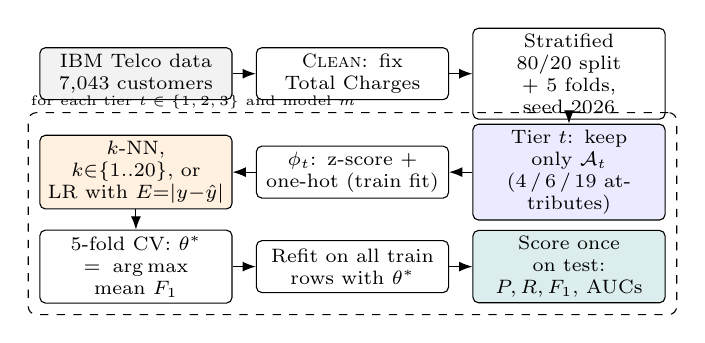
\begin{tikzpicture}[font=\scriptsize,
  box/.style={draw,rounded corners=2pt,align=center,inner sep=2pt,text width=2.3cm,minimum height=0.66cm},
  arr/.style={-Latex,thin}]
% row 1: shared data preparation (left to right)
\node[box,fill=black!5] (raw)   at (0,0)    {IBM Telco data\\$7{,}043$ customers};
\node[box]              (clean) at (2.75,0) {\textsc{Clean}: fix\\Total Charges};
\node[box]              (split) at (5.5,0)  {Stratified 80/20 split\\+ 5 folds, seed 2026};
% row 2: per tier and model (right to left)
\node[box,fill=blue!8]    (tier)  at (5.5,-1.25)  {Tier $t$: keep only $\mathcal{A}_t$\\(4\,/\,6\,/\,19 attributes)};
\node[box]                (enc)   at (2.75,-1.25) {$\phi_t$: z-score +\\one-hot (train fit)};
\node[box,fill=orange!12] (model) at (0,-1.25)    {$k$-NN, $k{\in}\{1..20\}$, or\\LR with $E{=}|y{-}\hat y|$};
% row 3: selection and evaluation (left to right)
\node[box]              (cv)    at (0,-2.45)    {5-fold CV: $\theta^*$\\$=\argmax$ mean $F_1$};
\node[box]              (refit) at (2.75,-2.45) {Refit on all train\\rows with $\theta^*$};
\node[box,fill=teal!14] (test)  at (5.5,-2.45)  {Score once on test:\\$P,R,F_1$, AUCs};
\draw[arr] (raw)--(clean); \draw[arr] (clean)--(split); \draw[arr] (split)--(tier);
\draw[arr] (tier)--(enc); \draw[arr] (enc)--(model); \draw[arr] (model)--(cv);
\draw[arr] (cv)--(refit); \draw[arr] (refit)--(test);
\node[draw,dashed,rounded corners=3pt,inner sep=4pt,fit=(tier)(model)(cv)(test)] (loop) {};
\node[anchor=south west,font=\tiny,inner sep=1pt] at (loop.north west) {for each tier $t\in\{1,2,3\}$ and model $m$};
\end{tikzpicture}
\caption{PRISM pipeline. Every tier and model share the same cleaned data, split and folds; a model only sees the attributes of its tier.}
\Description{Flowchart: raw data is cleaned and split; each of three nested tiers is encoded and passed to k-NN and logistic regression, tuned by 5-fold CV, refit on the training set and scored once on the test set.}\label{fig:pipeline}
\end{figure}

\section{Pseudo-code and Illustration}
Algorithm~\ref{alg:prism} gives the complete procedure, including the LR training routine, and Figure~\ref{fig:pipeline} illustrates the data flow. The tier loop is the experimental variable; everything inside it is identical across tiers, so differences in $\mathbf{q}_{m,t}$ can be attributed to the information available rather than to the protocol.

\section{Implementation}
\sloppy
The implementation follows the FAIR principles and the course's recommended structure. \texttt{src/main.py} runs Algorithm~\ref{alg:prism} end to end. Shared steps live in \texttt{src/cmn/}: \texttt{tiers.py} ($\mathcal{A}_t$), \texttt{data.py} (\textsc{Clean}, split, folds, $\phi_t$), \texttt{metrics.py} and \texttt{config.py} (seed, folds, paths). Each model has its own package: \texttt{src/knn/} for the $k$ sweep and \texttt{src/logistic\_regression/} for \textsc{Train}$_{\textsc{lr}}$, written directly in NumPy; \texttt{src/compare.py} writes the side-by-side table and chart. Results go to \texttt{output/<model>/} as CSV/JSON, and charts and analysis notebooks to \texttt{evaluation/}. A single \texttt{quickstart.sh} creates a virtual environment, installs the pinned \texttt{requirements.txt}, restores the dataset if missing, and runs the pipeline (under two minutes;\texttt{--fast} runs only $k$-NN). All randomness comes from seed $2026$, and each run records library versions in \texttt{output/run\_config.json}, so the same inputs and settings produce the same outputs.\par
\fussy

\begin{table}[t]
\caption{Selected settings and hold-out results from the current implementation (sanity run; full evaluation is Milestone~4).}\label{tab:run}
\small\setlength{\tabcolsep}{3.5pt}
\begin{tabular}{@{}llccc@{}}
\toprule
Tier & Model & $\theta^*$ & Test $F_1$ & ROC-AUC\\
\midrule
1 & $k$-NN & $k=15$ & 0.487 & 0.781\\
  & LR & $\eta{=}0.5,T{=}200,|B|{=}32$ & 0.538 & 0.782\\
2 & $k$-NN & $k=13$ & 0.580 & 0.815\\
  & LR & $\eta{=}0.5,T{=}200,|B|{=}32$ & 0.564 & 0.807\\
3 & $k$-NN & $k=19$ & 0.623 & 0.838\\
  & LR & $\eta{=}0.5,T{=}50,|B|{=}32$ & 0.621 & 0.842\\
\bottomrule
\end{tabular}
\end{table}

\bibliographystyle{ACM-Reference-Format}
\bibliography{bibliography}

\clearpage
\appendix
\section{AI Task Completion Disclosure (Category D)}
\textbf{AI use.} Claude (Anthropic) co-wrote the first LR experiment, merged the $k$-NN and LR work into one pipeline with shared code, a comparison step, README and quickstart, and drafted this report, including this appendix. OpenAI Codex fixed LR to the absolute-error loss, regenerated its results and renamed the loss. No AI use is recorded for the $k$-NN baseline. The team chose the design ($k$-NN baseline vs.\ LR, both taught in class) and kept the course loss function.

\subsection{Contributions and Evaluation of AI Output}
\sloppy
Drafted by Claude from the repository history; each member confirms their own statement.

\textbf{Abhishek Majumdar} set up the project and implemented the $k$-NN baseline: cleaning, 5-fold CV $k$ sweep, test evaluation and analysis plots. The AI restructure kept his cleaning rules, tiers and $k$ selection; run in the same environment, his original code and the restructured code give identical results.

\textbf{Dev Parsana} added instructor and TA access to the repository, and directed the AI-assisted integration of the $k$-NN and LR work into one pipeline, the shared-code restructure, the reproducibility re-run, the README and quickstart, and this report. He had the work audited against the manual, which found that \texttt{main} was outdated; the team overruled the AI's suggestion to drop the course loss.

\textbf{Ravi Vashi} added the earlier milestone files and implemented the LR experiment with grid search, later fixing it to the course loss. A tier document produced with AI stated the wrong seed and fill rule and was corrected; his updated LR results reproduce exactly with the pinned dependencies.
\end{document}
